% no page numbers for appendicies
\addtocontents{toc}{\protect\setcounter{tocdepth}{0}}
\addtocontents{toc}{\cftpagenumbersoff{chapter}}
\appendix
\titleformat{\chapter}{\normalfont\huge\bf}{Príloha \thechapter:}{1em}{}

\setcounter{figure}{0}
%\setcounter{listing}{0}
%\chapter{Technická dokumentácia}
%\pagenumbering{arabic}
%\renewcommand*{\thepage}{A-\arabic{page}}

% Harmonogram práce
\thispagestyle{empty}
\chapter{Harmonogram práce}
\pagenumbering{arabic}
\renewcommand*{\thepage}{A-\arabic{page}}
\section{Zimný semester}
\begin{table}[h!]
\renewcommand{\arraystretch}{1.3}
\begin{tabular}{|l|l|}
\hline
\textbf{Obdobie} & \textbf{Náplň práce}                                                                                                                                                                                                                         \\ \hline
1.týždeň         & Základný prehľad relevantnej literatúry.                                                                                                                                                                                                      \\ \hline
2.týždeň         & \begin{tabular}[c]{@{}l@{}}Štúdium literatúry ohľadom montorovania vibrácií. Pokusný zber dát \\ akcelerácie z MHD pomocou akcelerometra na smartfóne \\ a ich prieskumná analýza.\end{tabular}                                              \\ \hline
3.týždeň         & \begin{tabular}[c]{@{}l@{}}Štúdium článkov o frekvenčnej analýze a rešerš algoritmov \\ na hľadanie špičiek. Implementácia objavených prístupov hľadania \\ špičiek a aplikovanie na merania vibrácií z električiek a autobusu.\end{tabular} \\ \hline
4.týždeň         & Flashovanie firmvéru na vývojový kit iCOMOX.                                                                                                                                                                                                  \\ \hline
5.týždeň         & Osnova práce s referenciami na nájdenú literatúru.                                                                                                                                                                                            \\ \hline
6.týždeň         & \begin{tabular}[c]{@{}l@{}}Firmvér pre dosku na platforme ESP32 pre zaznám akceleračných \\ dát na SD kartu cez OpenLog\end{tabular}                                                                                                         \\ \hline
7.týždeň         & \begin{tabular}[c]{@{}l@{}}Merania vibrácií v MHD a analýza získaných záznamov v jupyter\\ notebooku. Doplnenie zdrojov pre časti osnovy s málo referenciami.\end{tabular}                                                                   \\ \hline
8.týždeň         & Sekcia 2.1. práce o monitorovaní vibrácií a šoku.                                                                                                                                                                                             \\ \hline
9.týždeň         & \begin{tabular}[c]{@{}l@{}}Doplnenie typov akcelerometov a časti o numerickej kvadratúre \\ k sekcii 2.1. Úvod do sekcie 2.2. o analýze v časovej doméne.\end{tabular}                                                                       \\ \hline
10.týždeň        & Deskriptívne štatistiky a algoritmy na identifikáciu špičiek.                                                                                                                                                                                 \\ \hline
11.týždeň        & Sekcia 2.2. o frekvenčnej a časovo-frekvenčnej analýze signálu.                                                                                                                                                                               \\ \hline
12.týždeň        & \begin{tabular}[c]{@{}l@{}}Sekcia 2.3 o architektúre senzorových sietí a ich obmedzeniach. \\ Návrh riešenia a úvod k priebežnej správe BP1\end{tabular}                                                                                     \\ \hline
13.týždeň        & Zapracované pripomienky k prezentovanému návrhu.                                                                                                                                                                             \\ \hline
\end{tabular}
\end{table}
\clearpage
\newpage
\section{Letný semester}
\begin{table}[h!]
\renewcommand{\arraystretch}{1.3}
\begin{tabular}{|l|l|}
\hline
\textbf{Obdobie} & \textbf{Orientačný plán práce}                                                                                                                                                       \\ \hline
1. -- 3. týždeň  & \begin{tabular}[c]{@{}l@{}}Odlaďovanie modelov na monitorovanie vibrácií na základe\\ analyzovaných algoritmov. Meranie úspešnosti na synteticky\\ generovaných dátach.\end{tabular} \\ \hline
4. -- 6. týždeň  & \begin{tabular}[c]{@{}l@{}}Návrh a prvotná implementácia firmvéru pre senzorovú jednotku\\ s loggovaním výstupných udalostí na pamäťovú kartu.\end{tabular}                          \\ \hline
7. -- 9. týždeň  & \begin{tabular}[c]{@{}l@{}}Optimalizácia posielaných dát cez zvolený bezdrôtový sieťový\\ protokol. Vzdialená konfigurácia zariadenia.\end{tabular}                                  \\ \hline
10 -- 13.týždeň  & \begin{tabular}[c]{@{}l@{}}Experimenty so senzorovou jednotkou v kontrolovanom\\ a reálnom prostredí. Vyhodnotenie výskumných otázok.\end{tabular}                                    \\ \hline
\end{tabular}
\end{table}

\thispagestyle{empty}

\chapter{Technická dokumentácia}
\pagenumbering{arabic}
\renewcommand*{\thepage}{B-\arabic{page}}

\section{Doxygen dokumentácia}
Po moduloch - hlavičkové súbory
- events.h  (events.c)
- inertial\_unit.h (inertial\_unit.c)
- peripheral.h  (peripheral.c)
- pipeline.h (pipeline.c, serialize.c, window.c)
- statistics.h (statistics.c)
Tasky: main.c

- Formát generovania syntetických dát

\section{MQTT topics a formát Message Pack správ}
imu/[id]/
- config/request
- config/response
- config/set

- login/set
- login/request
- login/response

- syslog
	"imu started"
	"config received"
	"config malformed"
	"config applied"
	"login malformed"
	"login saved"

- samples
\begin{verbatim}
[-0.07836493849754333, -0.9104690551757812, -9.964909553527832, -1.7736798524856567, -16.43988800048828, -0.4007977843284607, 1.4985052347183228, 5.201996326446533, 1.499103307723999]
\end{verbatim}

- stats/x, stats/y, stats/z
\begin{verbatim}
{"t": 386, "min": -9.964909553527832, "max": 11.8468656539917, "rms": 8.343297004699707, "avg": 4.126497745513916, "std": 7.251387119293213, "skew": -0.6144028306007385, "kurt": -0.8219752311706543, "med": 5.772983551025391, "mad": 5.370391845703125}
\end{verbatim}

- spectrum/x spectrum/y  spectrum/z
\begin{verbatim}
{"t": 25, "fs": 8, "bins": [0.0, -0.026730040088295937, -38.7723274230957, -38.19501495361328]}
\end{verbatim}

- events/x events/y events/z
\begin{verbatim}
{
"t": 386, "df": 2.0, 
"A": [{"i": 2, "t": 382, "d": 5, "h": -5.620919704437256}, {"i": 3, "t": 382, "d": 5, "h": -3.549427032470703}], 
"Z": []
}
\end{verbatim}

\begin{verbatim}
{"sensor": {"fs": 8, "range": "2g", "n": 8, "overlap": 0.5, "axis": [false, false, true]}, 
"tsmooth": {"on": false, "n": 8, "repeat": 1}, 
"stats": {"min": true, "max": true, "rms": true, "avg": true, "var": true, "std": true, "skew": true, "kurtosis": true, "med": true, "mad": true, "corr": false}, 
"transform": {"w": "hann", "f": "dft", "log": true},
"fsmooth": {"on": false, "n": 8, "repeat": 1},
"peak": {"tmin": 4, "tprox": 5, "strategy": "threshold", "threshold": {"t": -15.0},
"neighbours": {"k": 9, "e": 0.0, "h": -100.0, "h_rel": 10.0}, 
"zero_crossing": {"k": 4, "slope": 3.0}, 
"hill_walker": {"t": 0.0, "h": 0, "p": 10.0, "i": 3.0}}, 
"logger": {"local": false, "mqtt": true, "samples": "t", "stats": true, "events": true, "subsamp": 1}}
\end{verbatim}

\section{Datasety z premávky}
Typy vozidiel, trasy a umiestnenie zariadenia v každom z nich.
\begin{itemize}[noitemsep]
\item Električka Škoda 30 T 
\item Električka Škoda 29 T
\item Električka ČKD Tatra T6A5
\item Midibus Solaris Urbino 8,6
\item Elektrobus SOR NS 12 Electric
\item Kĺbový autobus Mercedes-Benz O 530 GL CapaCity
\end{itemize}

\thispagestyle{empty}

\chapter{Inštalačná a používateľská príručka}
\pagenumbering{arabic}
\renewcommand*{\thepage}{C-\arabic{page}}
Špecifikovať testovaciu platformu
(esp-idf) v4.4, FreeRTOS v9.0.0, esp-dsp v1.2, MPack v1.1, CMake - nástroj na automatizácie kompilácie (GNU 8.4.0), Platforma Manjaro Linux
	Linux ThinkPad 5.10.109-1-MANJARO (\url{https://ludocode.github.io/mpack/md_docs_expect.html}), Verzie a návod na inštaláciu v prílohe
- Python3.10, numpy, scipy (stats, signal, fft, interpolate), pandas, seaborn, matplotlib
- msgpack, json, cmd,  Eclipse Mosquitto

sudo pacman -S --needed gcc git make flex bison gperf python-pip cmake ninja ccache dfu-util libusb
\url{git clone -b v4.4 --recursive https://github.com/espressif/esp-idf.git}
\url{git clone -b v1.2.0 https://github.com/espressif/esp-dsp.git}
\url{wget https://github.com/ludocode/mpack/releases/download/v1.1/mpack-amalgamation-1.1.tar.gz}


cd ~/esp/esp-idf
./install.sh esp32


\textbf{Flashovanie a sprevádzkovanie}
. ./export.sh
cd firmware/vibration-analyzer
idf.py build
idf.py -p /dev/ttyUSB0 flash
idf.py -p /dev/ttyUSB0 monitor 

na SD kartu dať: config.txt


\textbf{MQTT klient na nahrávanie konfigurácií}
cd  main/tests/
pip install -r requirements.txt
python config\_tool.py

Príkazy:
	connect
		Device ID [1]:
      	Broker IP [192.168.1.103]
        Broker Port [1883]
	disconnect
	end
	^C
	
	set
		config>
	config
	topic
		topic>
		Listen time on topic in sec [10]:
	
	login
	credentials
	
\url{https://github.com/espressif/esp-idf}
\url{https://github.com/espressif/esp-dsp} s úpravou
\url{https://github.com/ludocode/mpack/releases/download/v1.1/mpack-amalgamation-1.1.tar.gz}

\textbf{Jupyter notebooky}
cd measurements
pip install -r requirements.txt
jupyter notebook

- Replikovateľnosť experimentov

	
\thispagestyle{empty}

\chapter{Vizualizácia datasetov}
\pagenumbering{arabic}
\renewcommand*{\thepage}{D-\arabic{page}}
\begin{figure}[h]
	\centering
	\begin{subfigure}{\textwidth}
        \centering
     	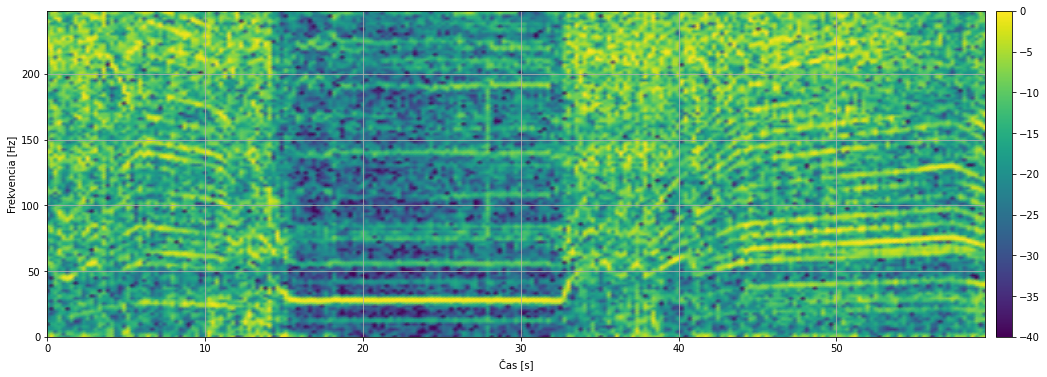
\includegraphics[width=\textwidth]{figures/verification/L83-dataset-spectrum.png}
     	\caption{Algoritmus č.1}
     \end{subfigure}
	\begin{subfigure}{\textwidth}
        \centering
     	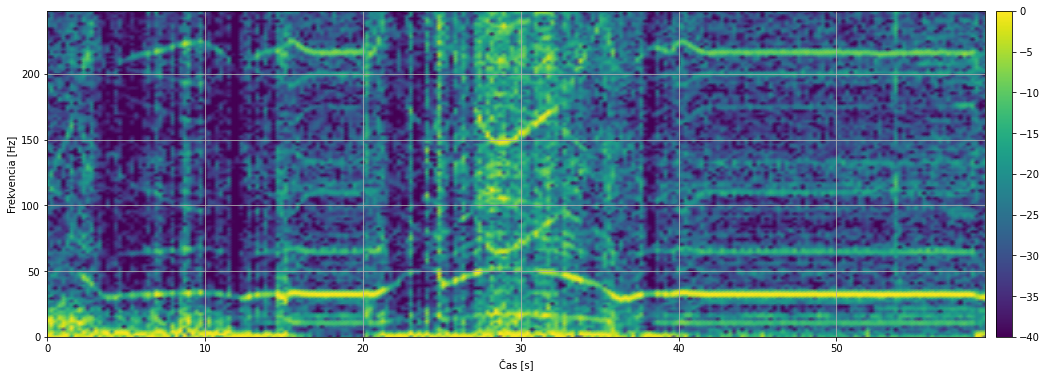
\includegraphics[width=\textwidth]{figures/verification/L35-dataset-spectrum.png}
     	\caption{Algoritmus č.1}
     \end{subfigure}
     \begin{subfigure}{\textwidth}
        \centering
     	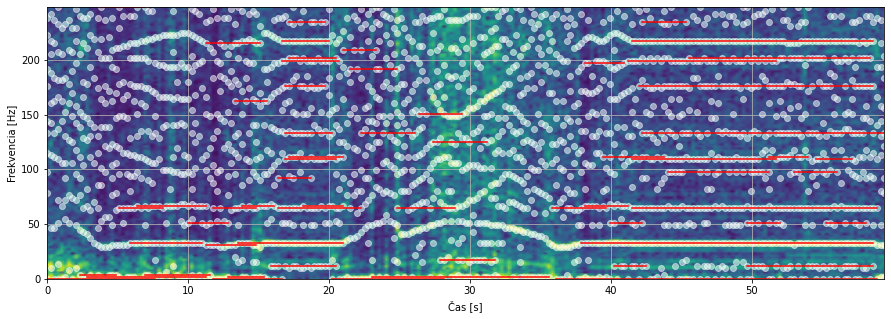
\includegraphics[width=\textwidth]{figures/verification/L35-dataset-A1.png}
     	\caption{Algoritmus č.1}
     \end{subfigure}
     \begin{subfigure}{\textwidth}
    	\centering
        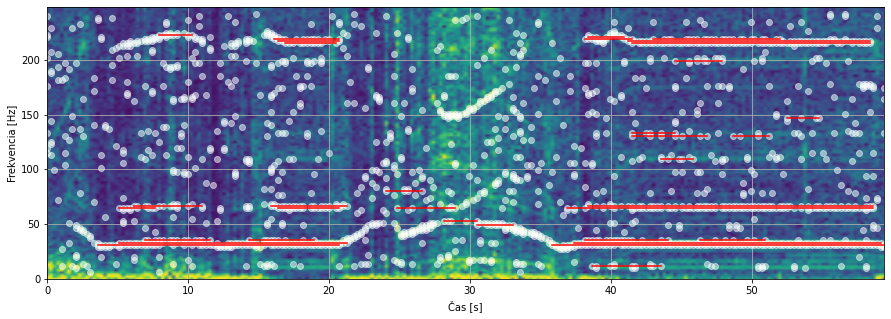
\includegraphics[width=\textwidth]{figures/verification/L35-dataset-A2.png}
        \caption{Algoritmus č.2}
     \end{subfigure}
      \begin{subfigure}{\textwidth}
    	\centering
        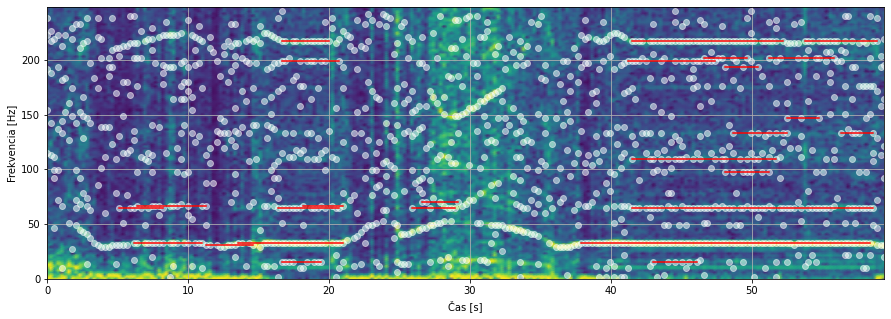
\includegraphics[width=\textwidth]{figures/verification/L35-dataset-A3.png}
        \caption{Algoritmus č.3}
     \end{subfigure}     
     \caption{L35 - Ilustrácia detegovaných špičiek pri fs 476Hz a N = 256 a parametrov podľa grid search}
\end{figure}

\chapter{Obsah digitálneho média}
\pagenumbering{arabic}
\renewcommand*{\thepage}{E-\arabic{page}}
\par Evidenčné číslo práce v informačnom systéme: \RegNo
\par Obsah digitálnej časti práce (archív ZIP):
\par Názov odovzdaného archívu: ...zip
\begin{verbatim}
> firmware
	> esp-dsp
	> esp-idf
	> mpack
	> vibration-analyzer
		> main
			> conf
			> docs
			> include
			> src
			> tests
> measurements
	> datasets
		> esp
		> synth-signal
	> experiments
	> signals
> BP_MiroslavHajek.pdf
\end{verbatim}


